\chapter{مبانی گراف}

بسیاری از مسائل برنامه‌نویسی با مدل‌سازی مسئله به عنوان یک مسئله گراف و استفاده از الگوریتم گرافی مناسب حل می‌شوند. یک مثال متداول از گراف، شبکه جاده‌ها و شهرهای یک کشور است. با این حال، گاهی گراف درون مسئله پنهان است و تشخیص آن دشوار خواهد بود.

این بخش از کتاب به بررسی الگوریتم‌های گراف می‌پردازد و تمرکز ویژه‌ای بر مباحث مهم در برنامه‌نویسی رقابتی دارد. در این فصل، مفاهیم مربوط به گراف‌ها را مرور کرده و روش‌های مختلف نمایش گراف در الگوریتم‌ها را بررسی می‌کنیم.

\section{اصطلاحات گراف}

\index{graph}
\index{node}
\index{edge}

یک \key{گراف} شامل \key{راس‌ها} (گره‌ها) و \key{یال‌ها} است. در این کتاب، متغیر $n$ بیانگر تعداد راس‌ها در گراف و متغیر $m$ نشان‌دهنده تعداد یال‌ها است. راس‌ها با اعداد صحیح $1,2,\ldots,n$ شماره‌گذاری می‌شوند.

برای نمونه، گراف زیر دارای ۵ راس و ۷ یال است:

\begin{center}
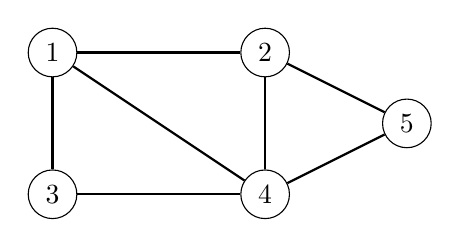
\begin{tikzpicture}[scale=0.9]
\node[draw, circle] (1) at (1,3) {$1$};
\node[draw, circle] (2) at (4,3) {$2$};
\node[draw, circle] (3) at (1,1) {$3$};
\node[draw, circle] (4) at (4,1) {$4$};
\node[draw, circle] (5) at (6,2) {$5$};

\path[draw,thick,-] (1) -- (2);
\path[draw,thick,-] (1) -- (3);
\path[draw,thick,-] (1) -- (4);
\path[draw,thick,-] (3) -- (4);
\path[draw,thick,-] (2) -- (4);
\path[draw,thick,-] (2) -- (5);
\path[draw,thick,-] (4) -- (5);
\end{tikzpicture}
\end{center}

\index{path}

یک \key{مسیر} از راس $a$ به راس $b$ از طریق یال‌های گراف حرکت می‌کند. \key{طول} مسیر برابر با تعداد یال‌های موجود در آن است. برای نمونه، گراف بالا شامل یک مسیر $1 \rightarrow 3 \rightarrow 4 \rightarrow 5$ با طول ۳ از راس ۱ به راس ۵ است:

\begin{center}
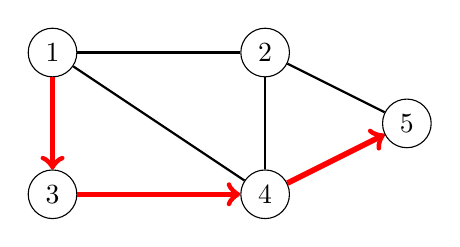
\begin{tikzpicture}[scale=0.9]
\node[draw, circle] (1) at (1,3) {$1$};
\node[draw, circle] (2) at (4,3) {$2$};
\node[draw, circle] (3) at (1,1) {$3$};
\node[draw, circle] (4) at (4,1) {$4$};
\node[draw, circle] (5) at (6,2) {$5$};

\path[draw,thick,-] (1) -- (2);
\path[draw,thick,-] (1) -- (3);
\path[draw,thick,-] (1) -- (4);
\path[draw,thick,-] (3) -- (4);
\path[draw,thick,-] (2) -- (4);
\path[draw,thick,-] (2) -- (5);
\path[draw,thick,-] (4) -- (5);

\path[draw=red,thick,->,line width=2pt] (1) -- (3);
\path[draw=red,thick,->,line width=2pt] (3) -- (4);
\path[draw=red,thick,->,line width=2pt] (4) -- (5);
\end{tikzpicture}
\end{center}

\index{cycle}

یک مسیر در صورتی یک \key{دور} است که راس اول و آخر آن یکسان باشد. برای نمونه، گراف بالا شامل دور $1 \rightarrow 3 \rightarrow 4 \rightarrow 1$ است. یک مسیر در صورتی \key{ساده} است که هر راس حداکثر یک بار در مسیر ظاهر شود.

% 
% \begin{itemize}
% \item $1 \rightarrow 2 \rightarrow 5$ (طول ۲)
% \item $1 \rightarrow 4 \rightarrow 5$ (طول ۲)
% \item $1 \rightarrow 2 \rightarrow 4 \rightarrow 5$ (طول ۳)
% \item $1 \rightarrow 3 \rightarrow 4 \rightarrow 5$ (طول ۳)
% \item $1 \rightarrow 4 \rightarrow 2 \rightarrow 5$ (طول ۳)
% \item $1 \rightarrow 3 \rightarrow 4 \rightarrow 2 \rightarrow 5$ (طول ۴)
% \end{itemize}

\subsubsection{همبندی}

\index{گراف همبند}

گراف \key{همبند} است اگر مسیری
بین هر دو رأس آن وجود داشته باشد.
برای نمونه، گراف زیر همبند است:
\begin{center}
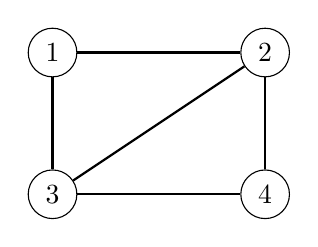
\begin{tikzpicture}[scale=0.9]
\node[draw, circle] (1) at (1,3) {$1$};
\node[draw, circle] (2) at (4,3) {$2$};
\node[draw, circle] (3) at (1,1) {$3$};
\node[draw, circle] (4) at (4,1) {$4$};
\path[draw,thick,-] (1) -- (2);
\path[draw,thick,-] (1) -- (3);
\path[draw,thick,-] (2) -- (3);
\path[draw,thick,-] (3) -- (4);
\path[draw,thick,-] (2) -- (4);
\end{tikzpicture}
\end{center}

گراف زیر ناهمبند است،
زیرا رفتن از رأس ۴
به هر رأس دیگری ممکن نیست:
\begin{center}
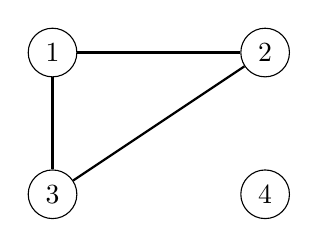
\begin{tikzpicture}[scale=0.9]
\node[draw, circle] (1) at (1,3) {$1$};
\node[draw, circle] (2) at (4,3) {$2$};
\node[draw, circle] (3) at (1,1) {$3$};
\node[draw, circle] (4) at (4,1) {$4$};
\path[draw,thick,-] (1) -- (2);
\path[draw,thick,-] (1) -- (3);
\path[draw,thick,-] (2) -- (3);
\end{tikzpicture}
\end{center}

\index{مؤلفه}

بخش‌های همبند گراف
\key{مؤلفه‌های} آن نامیده می‌شوند.
برای نمونه، گراف زیر
سه مؤلفه دارد:
$\{1,\,2,\,3\}$،
$\{4,\,5,\,6,\,7\}$ و
$\{8\}$.
\begin{center}
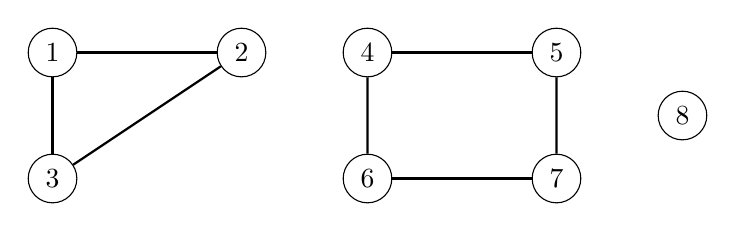
\begin{tikzpicture}[scale=0.8]
\node[draw, circle] (1) at (1,3) {$1$};
\node[draw, circle] (2) at (4,3) {$2$};
\node[draw, circle] (3) at (1,1) {$3$};

\node[draw, circle] (6) at (6,1) {$6$};
\node[draw, circle] (7) at (9,1) {$7$};
\node[draw, circle] (4) at (6,3) {$4$};
\node[draw, circle] (5) at (9,3) {$5$};

\node[draw, circle] (8) at (11,2) {$8$};

\path[draw,thick,-] (1) -- (2);
\path[draw,thick,-] (2) -- (3);
\path[draw,thick,-] (1) -- (3);
\path[draw,thick,-] (4) -- (5);
\path[draw,thick,-] (5) -- (7);
\path[draw,thick,-] (6) -- (7);
\path[draw,thick,-] (6) -- (4);
\end{tikzpicture}
\end{center}

\index{درخت}

\key{درخت} گرافی همبند
با $n$ رأس و $n-1$ یال است.
بین هر دو رأس درخت
دقیقاً یک مسیر یکتا وجود دارد.
برای نمونه، گراف زیر یک درخت است:

\begin{center}
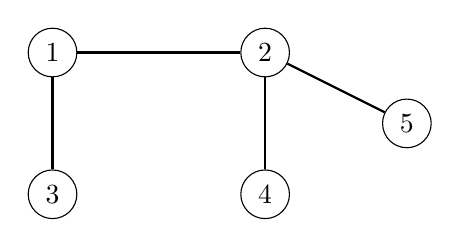
\begin{tikzpicture}[scale=0.9]
\node[draw, circle] (1) at (1,3) {$1$};
\node[draw, circle] (2) at (4,3) {$2$};
\node[draw, circle] (3) at (1,1) {$3$};
\node[draw, circle] (4) at (4,1) {$4$};
\node[draw, circle] (5) at (6,2) {$5$};

\path[draw,thick,-] (1) -- (2);
\path[draw,thick,-] (1) -- (3);
%\path[draw,thick,-] (1) -- (4);
\path[draw,thick,-] (2) -- (5);
\path[draw,thick,-] (2) -- (4);
%\path[draw,thick,-] (4) -- (5);
\end{tikzpicture}
\end{center}

\subsubsection{جهت یال‌ها}

\index{گراف جهت‌دار}

یک گراف \key{جهت‌دار} است
اگر یال‌ها تنها در یک جهت
قابل پیمایش باشند.
برای مثال، گراف زیر جهت‌دار است:
\begin{center}
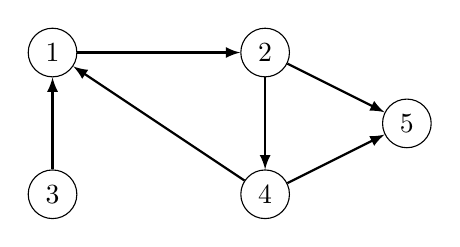
\begin{tikzpicture}[scale=0.9]
\node[draw, circle] (1) at (1,3) {$1$};
\node[draw, circle] (2) at (4,3) {$2$};
\node[draw, circle] (3) at (1,1) {$3$};
\node[draw, circle] (4) at (4,1) {$4$};
\node[draw, circle] (5) at (6,2) {$5$};
\path[draw,thick,->,>=latex] (1) -- (2);
\path[draw,thick,->,>=latex] (2) -- (4);
\path[draw,thick,->,>=latex] (2) -- (5);
\path[draw,thick,->,>=latex] (4) -- (5);
\path[draw,thick,->,>=latex] (4) -- (1);
\path[draw,thick,->,>=latex] (3) -- (1);
\end{tikzpicture}
\end{center}

گراف بالا شامل یک مسیر
$3 \rightarrow 1 \rightarrow 2 \rightarrow 5$
از گره $3$ به گره $5$ است،
اما هیچ مسیری از گره $5$ به گره $3$ وجود ندارد.

\subsubsection{وزن یال‌ها}

\index{گراف وزن‌دار}

در یک گراف \key{وزن‌دار}، به هر یال
یک \key{وزن} نسبت داده می‌شود.
وزن‌ها اغلب به عنوان طول یال تعبیر می‌شوند.
برای مثال، گراف زیر وزن‌دار است:
\begin{center}
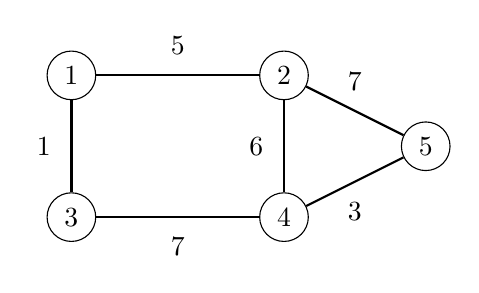
\begin{tikzpicture}[scale=0.9]
\node[draw, circle] (1) at (1,3) {$1$};
\node[draw, circle] (2) at (4,3) {$2$};
\node[draw, circle] (3) at (1,1) {$3$};
\node[draw, circle] (4) at (4,1) {$4$};
\node[draw, circle] (5) at (6,2) {$5$};
\path[draw,thick,-] (1) -- node[font=\small,label=above:5] {} (2);
\path[draw,thick,-] (1) -- node[font=\small,label=left:1] {} (3);
\path[draw,thick,-] (3) -- node[font=\small,label=below:7] {} (4);
\path[draw,thick,-] (2) -- node[font=\small,label=left:6] {} (4);
\path[draw,thick,-] (2) -- node[font=\small,label=above:7] {} (5);
\path[draw,thick,-] (4) -- node[font=\small,label=below:3] {} (5);
\end{tikzpicture}
\end{center}

طول یک مسیر در گراف وزن‌دار،
مجموع وزن یال‌های آن مسیر است.
برای مثال، در گراف بالا،
طول مسیر
$1 \rightarrow 2 \rightarrow 5$ برابر $12$ است،
و طول مسیر
$1 \rightarrow 3 \rightarrow 4 \rightarrow 5$ برابر $11$ است.
مسیر دوم، \key{کوتاه‌ترین} مسیر از گره $1$ به گره $5$ است.

\subsubsection{همسایه‌ها و درجه‌ها}

\index{همسایه}
\index{درجه}

دو گره \key{همسایه} یا \key{مجاور} هستند
اگر یالی بین آن‌ها وجود داشته باشد.
\key{درجه} یک گره
تعداد همسایه‌های آن است.
برای مثال، در گراف زیر،
همسایه‌های گره ۲ عبارت‌اند از ۱، ۴ و ۵،
بنابراین درجه آن ۳ است.

\begin{center}
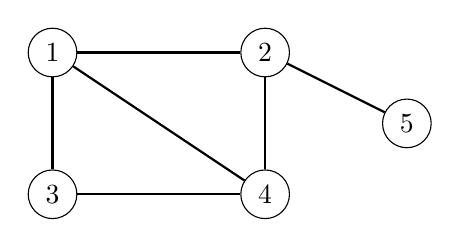
\begin{tikzpicture}[scale=0.9]
\node[draw, circle] (1) at (1,3) {$1$};
\node[draw, circle] (2) at (4,3) {$2$};
\node[draw, circle] (3) at (1,1) {$3$};
\node[draw, circle] (4) at (4,1) {$4$};
\node[draw, circle] (5) at (6,2) {$5$};

\path[draw,thick,-] (1) -- (2);
\path[draw,thick,-] (1) -- (3);
\path[draw,thick,-] (1) -- (4);
\path[draw,thick,-] (3) -- (4);
\path[draw,thick,-] (2) -- (4);
\path[draw,thick,-] (2) -- (5);
%\path[draw,thick,-] (4) -- (5);
\end{tikzpicture}
\end{center}

مجموع درجات در گراف همیشه $2m$ است؛
$m$ تعداد یال‌ها است،
زیرا هر یال
درجه دقیقاً دو رأس را یک واحد افزایش می‌دهد.
به همین دلیل، مجموع درجات همیشه زوج است.

\index{گراف منتظم}
\index{گراف کامل}

گراف \key{منتظم} است اگر
درجه هر رأس مقدار ثابت $d$ باشد.
گراف \key{کامل} است اگر
درجه هر رأس $n-1$ باشد؛ یعنی
گراف شامل تمام یال‌های ممکن
بین رأس‌ها است.

\index{درجه ورودی}
\index{درجه خروجی}

در گراف جهت‌دار، \key{درجه ورودی}
یک رأس برابر با تعداد یال‌هایی است
که به آن رأس ختم می‌شوند،
و \key{درجه خروجی} یک رأس
برابر با تعداد یال‌هایی است که از آن رأس آغاز می‌شوند.
برای نمونه، در گراف زیر،
درجه ورودی رأس ۲ برابر ۲،
و درجه خروجی رأس ۲ برابر ۱ است.

\begin{center}
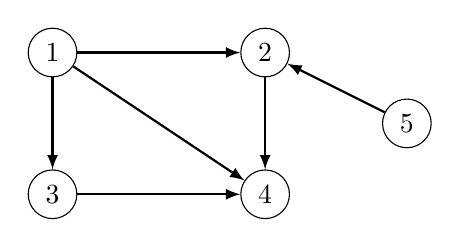
\begin{tikzpicture}[scale=0.9]
\node[draw, circle] (1) at (1,3) {$1$};
\node[draw, circle] (2) at (4,3) {$2$};
\node[draw, circle] (3) at (1,1) {$3$};
\node[draw, circle] (4) at (4,1) {$4$};
\node[draw, circle] (5) at (6,2) {$5$};

\path[draw,thick,->,>=latex] (1) -- (2);
\path[draw,thick,->,>=latex] (1) -- (3);
\path[draw,thick,->,>=latex] (1) -- (4);
\path[draw,thick,->,>=latex] (3) -- (4);
\path[draw,thick,->,>=latex] (2) -- (4);
\path[draw,thick,<-,>=latex] (2) -- (5);
\end{tikzpicture}
\end{center}

\subsubsection{رنگ‌آمیزی‌ها}

\index{رنگ‌آمیزی}
\index{گراف دوپخش}

در \key{رنگ‌آمیزی} گراف،
به هر رأس رنگی تخصیص داده می‌شود به گونه‌ای که
هیچ دو رأس مجاوری رنگ یکسان نداشته باشند.

یک گراف \key{دوبخشی} (یا دوپاره) است اگر
بتوان آن را با دو رنگ، رنگ‌آمیزی کرد.
مشخص شده است که یک گراف دوبخشی است
دقیقاً زمانی که هیچ دوری با تعداد یال‌های
فرد نداشته باشد.
برای مثال، گراف
\begin{center}
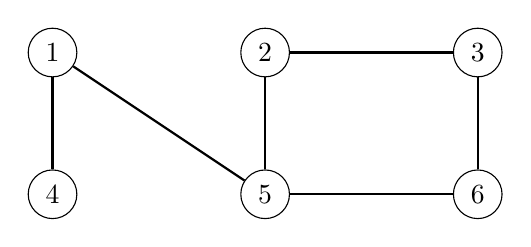
\begin{tikzpicture}[scale=0.9]
\node[draw, circle] (1) at (1,3) {$2$};
\node[draw, circle] (2) at (4,3) {$3$};
\node[draw, circle] (3) at (1,1) {$5$};
\node[draw, circle] (4) at (4,1) {$6$};
\node[draw, circle] (5) at (-2,1) {$4$};
\node[draw, circle] (6) at (-2,3) {$1$};
\path[draw,thick,-] (1) -- (2);
\path[draw,thick,-] (1) -- (3);
\path[draw,thick,-] (3) -- (4);
\path[draw,thick,-] (2) -- (4);
\path[draw,thick,-] (3) -- (6);
\path[draw,thick,-] (5) -- (6);
\end{tikzpicture}
\end{center}
دوبخشی است، زیرا می‌توان آن را به شکل زیر رنگ‌آمیزی کرد:
\begin{center}
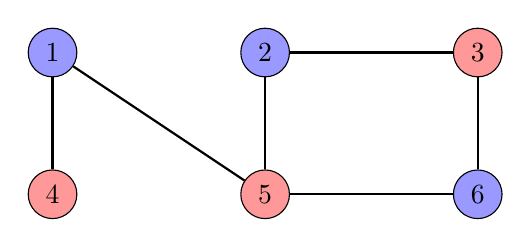
\begin{tikzpicture}[scale=0.9]
\node[draw, circle, fill=blue!40] (1) at (1,3) {$2$};
\node[draw, circle, fill=red!40] (2) at (4,3) {$3$};
\node[draw, circle, fill=red!40] (3) at (1,1) {$5$};
\node[draw, circle, fill=blue!40] (4) at (4,1) {$6$};
\node[draw, circle, fill=red!40] (5) at (-2,1) {$4$};
\node[draw, circle, fill=blue!40] (6) at (-2,3) {$1$};
\path[draw,thick,-] (1) -- (2);
\path[draw,thick,-] (1) -- (3);
\path[draw,thick,-] (3) -- (4);
\path[draw,thick,-] (2) -- (4);
\path[draw,thick,-] (3) -- (6);
\path[draw,thick,-] (5) -- (6);
\end{tikzpicture}
\end{center}
اما گراف زیر
\begin{center}
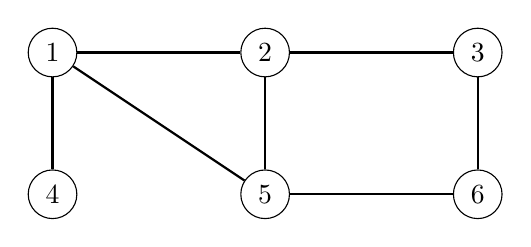
\begin{tikzpicture}[scale=0.9]
\node[draw, circle] (1) at (1,3) {$2$};
\node[draw, circle] (2) at (4,3) {$3$};
\node[draw, circle] (3) at (1,1) {$5$};
\node[draw, circle] (4) at (4,1) {$6$};
\node[draw, circle] (5) at (-2,1) {$4$};
\node[draw, circle] (6) at (-2,3) {$1$};
\path[draw,thick,-] (1) -- (2);
\path[draw,thick,-] (1) -- (3);
\path[draw,thick,-] (3) -- (4);
\path[draw,thick,-] (2) -- (4);
\path[draw,thick,-] (3) -- (6);
\path[draw,thick,-] (5) -- (6);
\path[draw,thick,-] (1) -- (6);
\end{tikzpicture}
\end{center}
دوبخشی نیست، زیرا نمی‌توان دور سه رأسی
زیر را با دو رنگ، رنگ‌آمیزی کرد:
\begin{center}
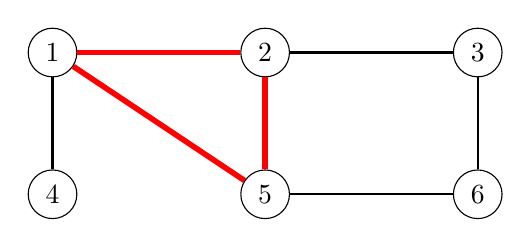
\begin{tikzpicture}[scale=0.9]
\node[draw, circle] (1) at (1,3) {$2$};
\node[draw, circle] (2) at (4,3) {$3$};
\node[draw, circle] (3) at (1,1) {$5$};
\node[draw, circle] (4) at (4,1) {$6$};
\node[draw, circle] (5) at (-2,1) {$4$};
\node[draw, circle] (6) at (-2,3) {$1$};
\path[draw,thick,-] (1) -- (2);
\path[draw,thick,-] (1) -- (3);
\path[draw,thick,-] (3) -- (4);
\path[draw,thick,-] (2) -- (4);
\path[draw,thick,-] (3) -- (6);
\path[draw,thick,-] (5) -- (6);
\path[draw,thick,-] (1) -- (6);

\path[draw=red,thick,-,line width=2pt] (1) -- (3);
\path[draw=red,thick,-,line width=2pt] (3) -- (6);
\path[draw=red,thick,-,line width=2pt] (6) -- (1);
\end{tikzpicture}
\end{center}

\subsubsection{ساده بودن}

\index{گراف ساده}

یک گراف \key{ساده} است
اگر هیچ یالی در یک رأس شروع و پایان نیابد،
و هیچ یال چندگانه‌ای
بین دو رأس وجود نداشته باشد.
اغلب فرض می‌کنیم گراف‌ها ساده هستند.
به‌عنوان مثال، گراف زیر ساده \emph{نیست}:
\begin{center}
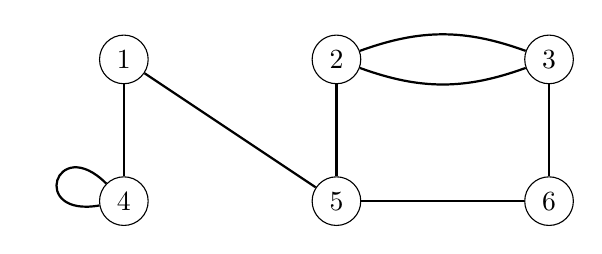
\begin{tikzpicture}[scale=0.9]
\node[draw, circle] (1) at (1,3) {$2$};
\node[draw, circle] (2) at (4,3) {$3$};
\node[draw, circle] (3) at (1,1) {$5$};
\node[draw, circle] (4) at (4,1) {$6$};
\node[draw, circle] (5) at (-2,1) {$4$};
\node[draw, circle] (6) at (-2,3) {$1$};

\path[draw,thick,-] (1) edge [bend right=20] (2);
\path[draw,thick,-] (2) edge [bend right=20] (1);
%\path[draw,thick,-] (1) -- (2);
\path[draw,thick,-] (1) -- (3);
\path[draw,thick,-] (3) -- (4);
\path[draw,thick,-] (2) -- (4);
\path[draw,thick,-] (3) -- (6);
\path[draw,thick,-] (5) -- (6);

\tikzset{every loop/.style={in=135,out=190}}
\path[draw,thick,-] (5) edge [loop left] (5);
\end{tikzpicture}
\end{center}

\section{نمایش گراف}

روش‌های متعددی برای نمایش گراف‌ها
در الگوریتم‌ها وجود دارد.
انتخاب ساختمان داده
به اندازه گراف و
نحوه پردازش آن توسط الگوریتم بستگی دارد.
در ادامه سه نمایش متداول را بررسی می‌کنیم.

\subsubsection{نمایش لیست مجاورت}

\index{adjacency list}

در نمایش لیست مجاورت،
به هر رأس $x$ در گراف یک \key{لیست مجاورت} تخصیص داده می‌شود
که شامل رأس‌هایی است
که یالی از $x$ به آن‌ها وجود دارد.
لیست‌های مجاورت محبوب‌ترین روش
برای نمایش گراف‌ها هستند و اغلب الگوریتم‌ها را می‌توان
به‌طور کارآمد با استفاده از آن‌ها پیاده‌سازی کرد.

روش مناسب برای ذخیره لیست‌های مجاورت، تعریف
یک آرایه از بردارها به صورت زیر است:
\begin{lstlisting}
vector<int> adj[N];
\end{lstlisting}

مقدار ثابت $N$ طوری انتخاب می‌شود که تمام
لیست‌های مجاورت قابل ذخیره‌سازی باشند.
به‌عنوان مثال، گراف

\begin{center}
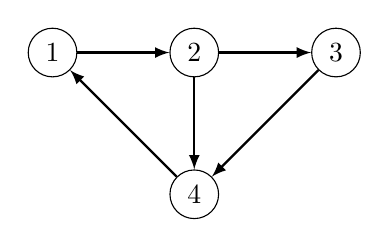
\begin{tikzpicture}[scale=0.9]
\node[draw, circle] (1) at (1,3) {$1$};
\node[draw, circle] (2) at (3,3) {$2$};
\node[draw, circle] (3) at (5,3) {$3$};
\node[draw, circle] (4) at (3,1) {$4$};

\path[draw,thick,->,>=latex] (1) -- (2);
\path[draw,thick,->,>=latex] (2) -- (3);
\path[draw,thick,->,>=latex] (2) -- (4);
\path[draw,thick,->,>=latex] (3) -- (4);
\path[draw,thick,->,>=latex] (4) -- (1);
\end{tikzpicture}
\end{center}
می‌تواند به این صورت ذخیره شود:
\begin{lstlisting}
adj[1].push_back(2);
adj[2].push_back(3);
adj[2].push_back(4);
adj[3].push_back(4);
adj[4].push_back(1);
\end{lstlisting}

اگر گراف بدون جهت باشد، می‌توان آن را به شکل مشابه ذخیره کرد،
اما هر یال در هر دو جهت اضافه می‌شود.

برای یک گراف وزن‌دار، ساختار را می‌توان
به صورت زیر گسترش داد:

\begin{lstlisting}
vector<pair<int,int>> adj[N];
\end{lstlisting}

در این حالت، لیست مجاورت رأس $a$
شامل جفت $(b,w)$ است
هر زمان که یالی از رأس $a$ به رأس $b$
با وزن $w$ وجود داشته باشد. به‌عنوان مثال، گراف

\begin{center}
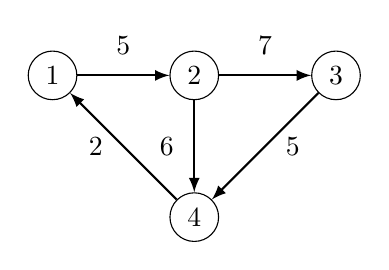
\begin{tikzpicture}[scale=0.9]
\node[draw, circle] (1) at (1,3) {$1$};
\node[draw, circle] (2) at (3,3) {$2$};
\node[draw, circle] (3) at (5,3) {$3$};
\node[draw, circle] (4) at (3,1) {$4$};

\path[draw,thick,->,>=latex] (1) -- node[font=\small,label=above:5] {} (2);
\path[draw,thick,->,>=latex] (2) -- node[font=\small,label=above:7] {} (3);
\path[draw,thick,->,>=latex] (2) -- node[font=\small,label=left:6] {} (4);
\path[draw,thick,->,>=latex] (3) -- node[font=\small,label=right:5] {} (4);
\path[draw,thick,->,>=latex] (4) -- node[font=\small,label=left:2] {} (1);
\end{tikzpicture}
\end{center}
می‌تواند به صورت زیر ذخیره شود:
\begin{lstlisting}
adj[1].push_back({2,5});
adj[2].push_back({3,7});
adj[2].push_back({4,6});
adj[3].push_back({4,5});
adj[4].push_back({1,2});
\end{lstlisting}

مزیت استفاده از لیست‌های مجاورت این است که
می‌توان به شکل کارآمد گره‌هایی را یافت که
از یک گره مفروض با یک یال قابل دسترسی هستند.
برای نمونه، حلقه زیر روی تمام گره‌هایی پیمایش می‌کند
که از گره $s$ قابل دسترسی‌اند:

\begin{lstlisting}
for (auto u : adj[s]) {
    // پردازش گره u
}
\end{lstlisting}

\subsubsection{نمایش ماتریس مجاورت}

\index{ماتریس مجاورت}

یک \key{ماتریس مجاورت} آرایه‌ای دوبعدی است
که نشان می‌دهد گراف شامل چه یال‌هایی است.
می‌توان از ماتریس مجاورت وجود یال بین دو گره را
به صورت کارآمد بررسی کرد.
این ماتریس می‌تواند به شکل آرایه‌ای ذخیره شود:
\begin{lstlisting}
int adj[N][N];
\end{lstlisting}
که در آن هر مقدار $\texttt{adj}[a][b]$ نشان می‌دهد
آیا گراف شامل یالی از گره $a$ به گره $b$ است یا خیر.
اگر یال در گراف وجود داشته باشد،
$\texttt{adj}[a][b]=1$
و در غیر این صورت $\texttt{adj}[a][b]=0$ خواهد بود.
برای نمونه، گراف
\begin{center}
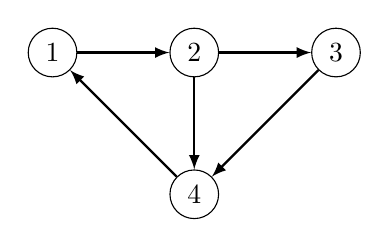
\begin{tikzpicture}[scale=0.9]
\node[draw, circle] (1) at (1,3) {$1$};
\node[draw, circle] (2) at (3,3) {$2$};
\node[draw, circle] (3) at (5,3) {$3$};
\node[draw, circle] (4) at (3,1) {$4$};

\path[draw,thick,->,>=latex] (1) -- (2);
\path[draw,thick,->,>=latex] (2) -- (3);
\path[draw,thick,->,>=latex] (2) -- (4);
\path[draw,thick,->,>=latex] (3) -- (4);
\path[draw,thick,->,>=latex] (4) -- (1);
\end{tikzpicture}
\end{center}
می‌تواند به صورت زیر نمایش داده شود:
\begin{center}
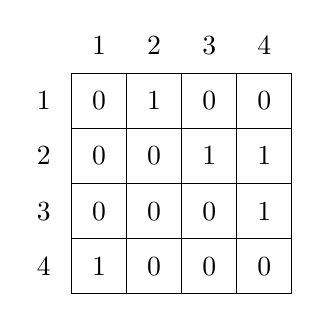
\begin{tikzpicture}[scale=0.7]
\draw (0,0) grid (4,4);
\node at (0.5,0.5) {1};
\node at (1.5,0.5) {0};
\node at (2.5,0.5) {0};
\node at (3.5,0.5) {0};
\node at (0.5,1.5) {0};
\node at (1.5,1.5) {0};
\node at (2.5,1.5) {0};
\node at (3.5,1.5) {1};
\node at (0.5,2.5) {0};
\node at (1.5,2.5) {0};
\node at (2.5,2.5) {1};
\node at (3.5,2.5) {1};
\node at (0.5,3.5) {0};
\node at (1.5,3.5) {1};
\node at (2.5,3.5) {0};
\node at (3.5,3.5) {0};
\node at (-0.5,0.5) {4};
\node at (-0.5,1.5) {3};
\node at (-0.5,2.5) {2};
\node at (-0.5,3.5) {1};
\node at (0.5,4.5) {1};
\node at (1.5,4.5) {2};
\node at (2.5,4.5) {3};
\node at (3.5,4.5) {4};
\end{tikzpicture}
\end{center}

اگر گراف وزن‌دار باشد، نمایش ماتریس مجاورت
می‌تواند تعمیم یابد تا در صورت وجود یال،
ماتریس حاوی وزن آن یال باشد.
با استفاده از این نمایش، گراف

\begin{center}
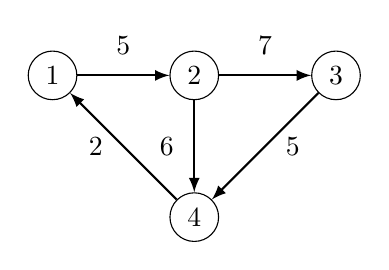
\begin{tikzpicture}[scale=0.9]
\node[draw, circle] (1) at (1,3) {$1$};
\node[draw, circle] (2) at (3,3) {$2$};
\node[draw, circle] (3) at (5,3) {$3$};
\node[draw, circle] (4) at (3,1) {$4$};

\path[draw,thick,->,>=latex] (1) -- node[font=\small,label=above:5] {} (2);
\path[draw,thick,->,>=latex] (2) -- node[font=\small,label=above:7] {} (3);
\path[draw,thick,->,>=latex] (2) -- node[font=\small,label=left:6] {} (4);
\path[draw,thick,->,>=latex] (3) -- node[font=\small,label=right:5] {} (4);
\path[draw,thick,->,>=latex] (4) -- node[font=\small,label=left:2] {} (1);
\end{tikzpicture}
\end{center}
\begin{samepage}
با ماتریس زیر متناظر است:
\begin{center}
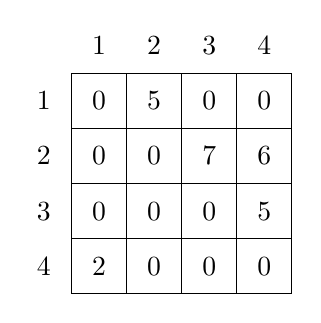
\begin{tikzpicture}[scale=0.7]
\draw (0,0) grid (4,4);
\node at (0.5,0.5) {2};
\node at (1.5,0.5) {0};
\node at (2.5,0.5) {0};
\node at (3.5,0.5) {0};
\node at (0.5,1.5) {0};
\node at (1.5,1.5) {0};
\node at (2.5,1.5) {0};
\node at (3.5,1.5) {5};
\node at (0.5,2.5) {0};
\node at (1.5,2.5) {0};
\node at (2.5,2.5) {7};
\node at (3.5,2.5) {6};
\node at (0.5,3.5) {0};
\node at (1.5,3.5) {5};
\node at (2.5,3.5) {0};
\node at (3.5,3.5) {0};
\node at (-0.5,0.5) {4};
\node at (-0.5,1.5) {3};
\node at (-0.5,2.5) {2};
\node at (-0.5,3.5) {1};
\node at (0.5,4.5) {1};
\node at (1.5,4.5) {2};
\node at (2.5,4.5) {3};
\node at (3.5,4.5) {4};
\end{tikzpicture}
\end{center}
\end{samepage}

عیب نمایش ماتریس مجاورت
وجود $n^2$ عنصر است
که اغلب صفر هستند.
به همین دلیل گراف بزرگ باشد
این نمایش قابل استفاده نیست.

\subsubsection{نمایش فهرست یال‌ها}

\index{فهرست یال‌ها}

یک \key{فهرست یال} تمام یال‌های گراف را
با ترتیبی دلخواه نگه می‌دارد.
روش مناسبی است
اگر الگوریتم همه یال‌ها را پیمایش کند
و نیازی به یافتن یال‌های خروجی از یک رأس خاص نباشد.

فهرست یال‌ها را می‌توان در یک بردار ذخیره کرد:
\begin{lstlisting}
vector<pair<int,int>> edges;
\end{lstlisting}
که در آن هر جفت $(a,b)$ نشان‌دهنده
یالی از رأس $a$ به رأس $b$ است.
بنابراین، گراف

\begin{center}
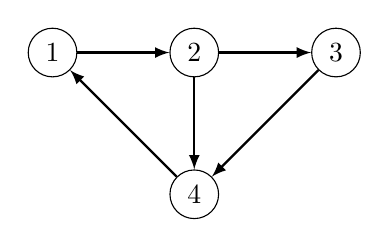
\begin{tikzpicture}[scale=0.9]
\node[draw, circle] (1) at (1,3) {$1$};
\node[draw, circle] (2) at (3,3) {$2$};
\node[draw, circle] (3) at (5,3) {$3$};
\node[draw, circle] (4) at (3,1) {$4$};

\path[draw,thick,->,>=latex] (1) -- (2);
\path[draw,thick,->,>=latex] (2) -- (3);
\path[draw,thick,->,>=latex] (2) -- (4);
\path[draw,thick,->,>=latex] (3) -- (4);
\path[draw,thick,->,>=latex] (4) -- (1);
\end{tikzpicture}
\end{center}
به شکل زیر نمایش داده می‌شود:
\begin{lstlisting}
edges.push_back({1,2});
edges.push_back({2,3});
edges.push_back({2,4});
edges.push_back({3,4});
edges.push_back({4,1});
\end{lstlisting}

\noindent
اگر گراف وزن‌دار باشد، ساختار داده بدین صورت
گسترش می‌یابد:
\begin{lstlisting}
vector<tuple<int,int,int>> edges;
\end{lstlisting}
هر عضو در این فهرست به فرم $(a,b,w)$ است
که بیانگر یالی از رأس $a$ به رأس $b$ با وزن $w$ است.
برای نمونه، گراف

\begin{center}
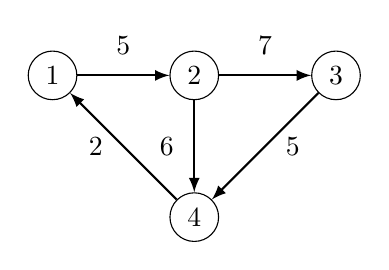
\begin{tikzpicture}[scale=0.9]
\node[draw, circle] (1) at (1,3) {$1$};
\node[draw, circle] (2) at (3,3) {$2$};
\node[draw, circle] (3) at (5,3) {$3$};
\node[draw, circle] (4) at (3,1) {$4$};

\path[draw,thick,->,>=latex] (1) -- node[font=\small,label=above:5] {} (2);
\path[draw,thick,->,>=latex] (2) -- node[font=\small,label=above:7] {} (3);
\path[draw,thick,->,>=latex] (2) -- node[font=\small,label=left:6] {} (4);
\path[draw,thick,->,>=latex] (3) -- node[font=\small,label=right:5] {} (4);
\path[draw,thick,->,>=latex] (4) -- node[font=\small,label=left:2] {} (1);
\end{tikzpicture}
\end{center}
\begin{samepage}
می‌تواند به صورت زیر نمایش داده شود\footnote{در برخی کامپایلرهای قدیمی‌تر، باید از تابع
\texttt{make\_tuple} به جای آکولاد استفاده شود (برای مثال،
\texttt{make\_tuple(1,2,5)} به جای \texttt{\{1,2,5\}}).}:
\begin{lstlisting}
edges.push_back({1,2,5});
edges.push_back({2,3,7});
edges.push_back({2,4,6});
edges.push_back({3,4,5});
edges.push_back({4,1,2});
\end{lstlisting}
\end{samepage}